\section{Background} \label{sec:background}

%\begin{figure}[t!] 
%\begin{minipage}{1\linewidth}
%\begin{subfigure}[c]{0.96\linewidth}
%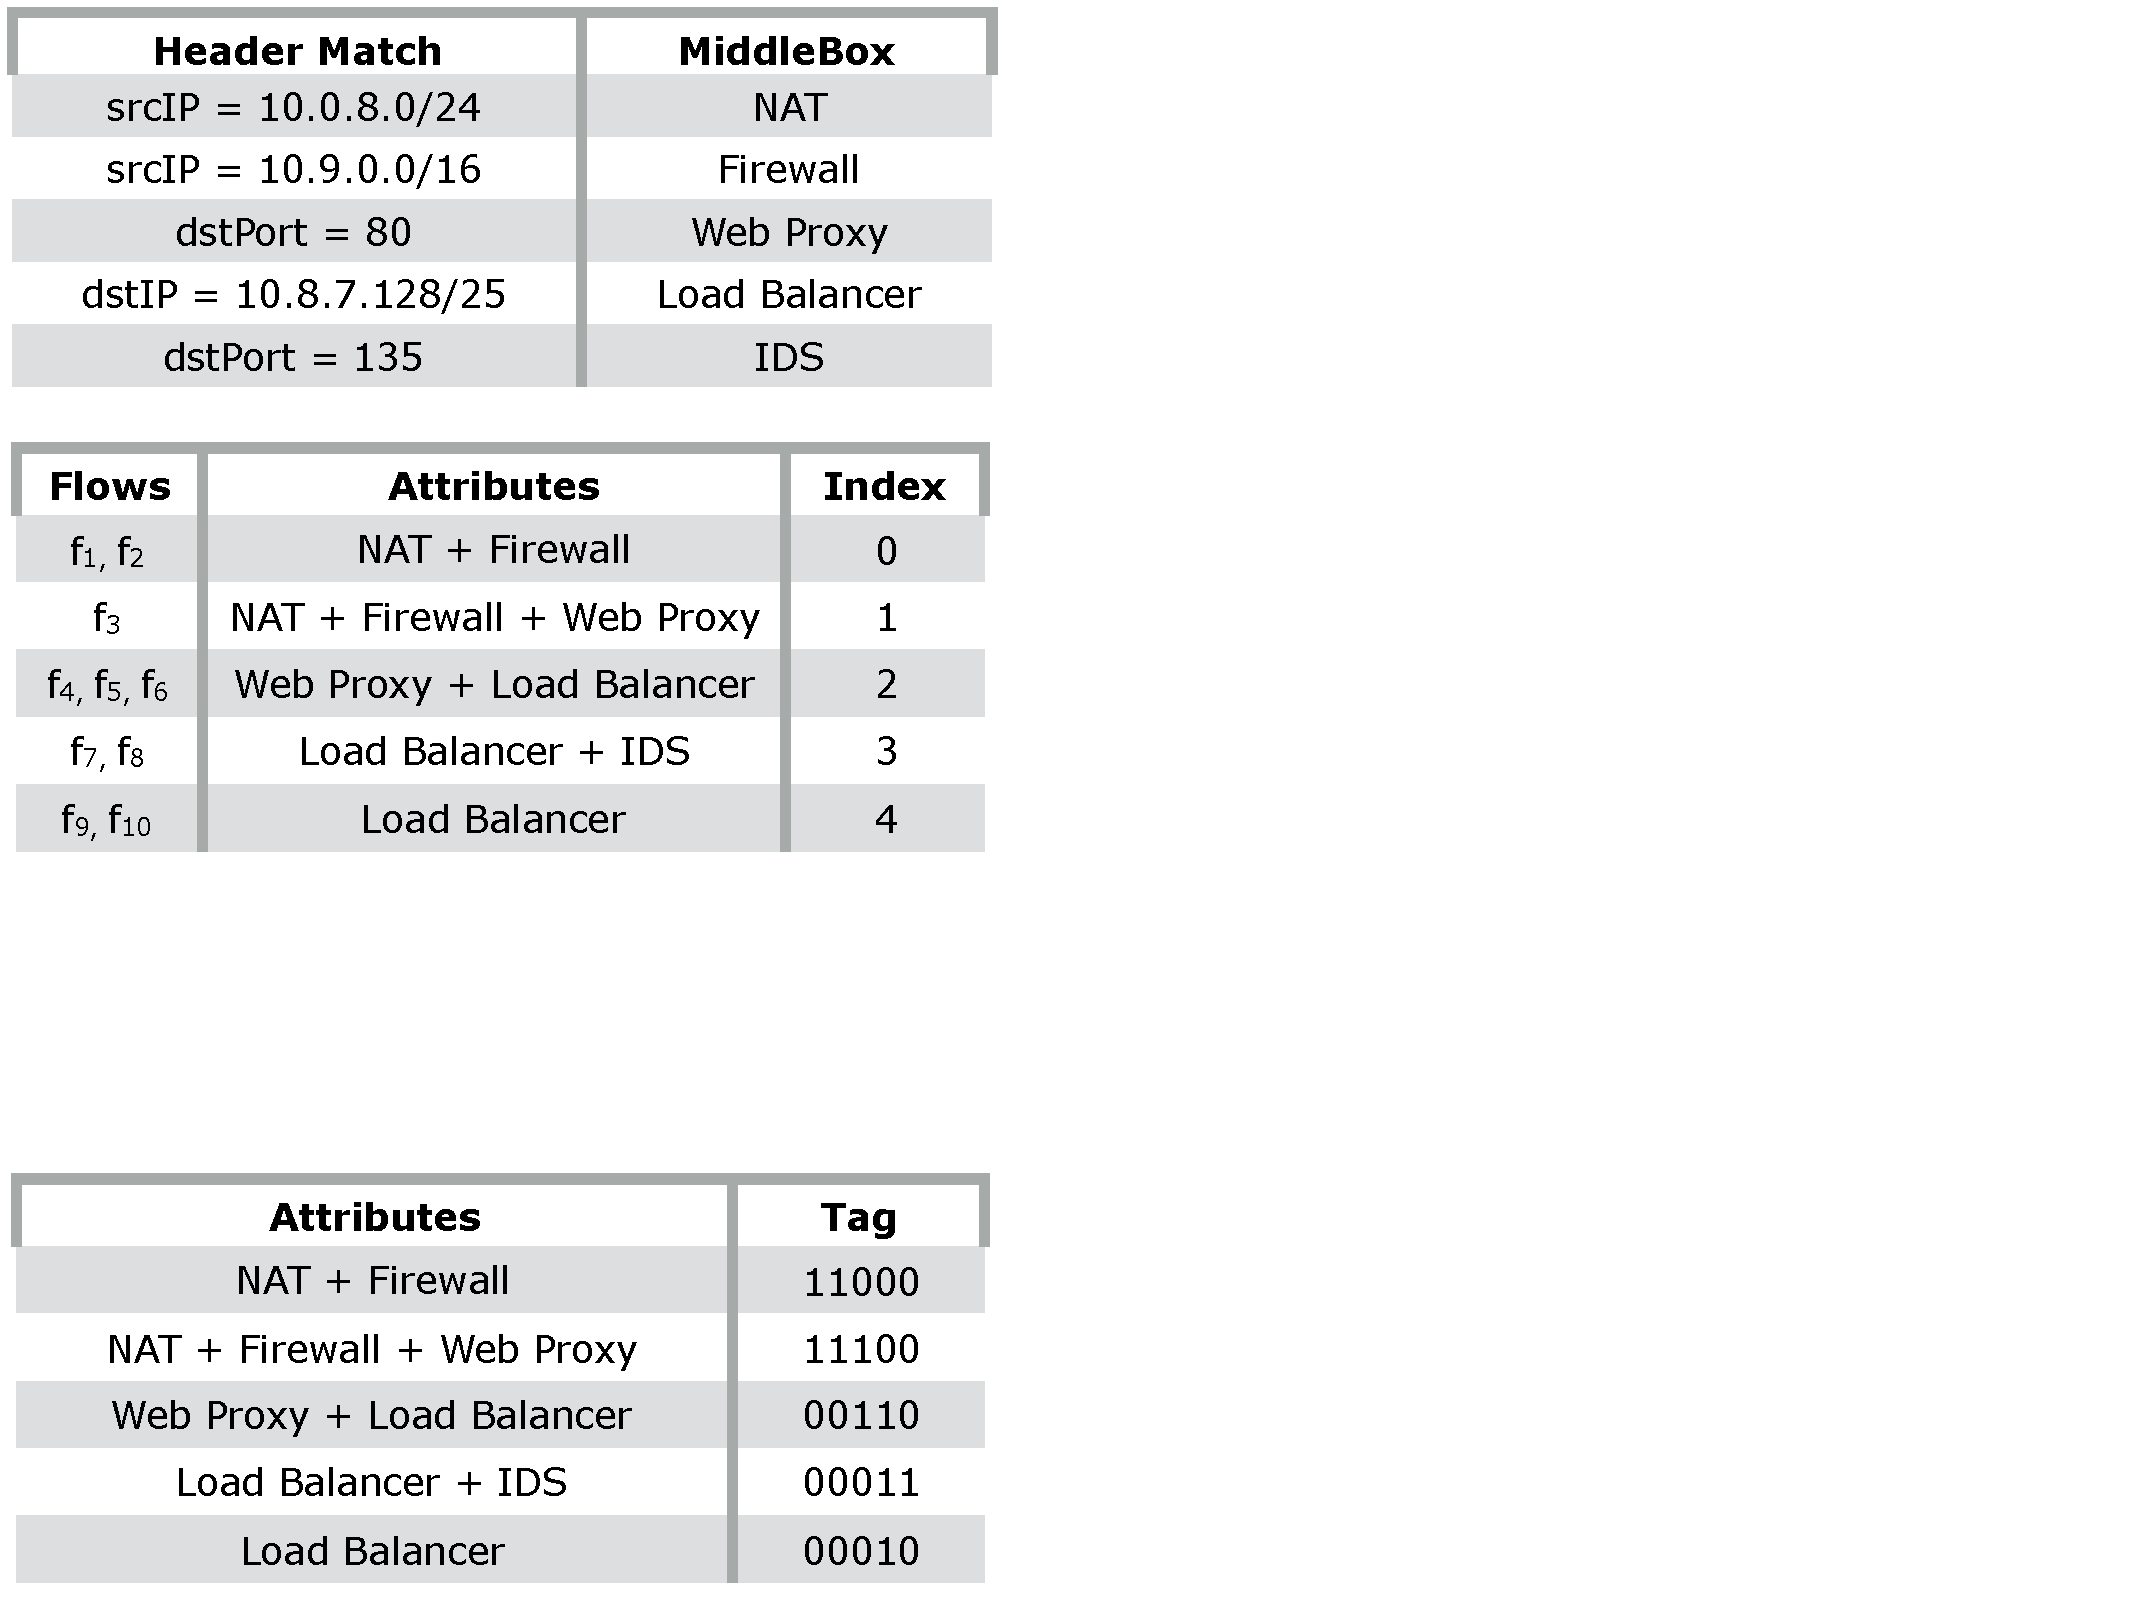
\includegraphics[trim={0 12cm 19cm 0}, clip, width=\linewidth]{figures/mbox_path_example3}
%\end{subfigure} 
%\end{minipage} 
%\caption{In this example, we have a policy that defines traffic which must flow through subsets of five middleboxes. The first table shows which header fields trigger each middlebox, and the second table shows some combinations we may see in network traffic. }
%\label{fig:mbox_policies}
%\end{figure}

\begin{figure}
    \begin{tabular}{| p{2.5cm} | p{2cm} | p{2cm} |}
    \hline
    Tagging Application & FEC-Defining Attributes & Ordered Attributes?\\ \hline
    SDN-Enabled IXP & Advertising Peers & No \\ \hline
    Service Chaining & Middleboxes& Yes \\ \hline
    Policy Enforcement & Host Permissions & No \\ \hline
    Multicast/Anycast & Destination Hosts & Maybe \\
    \hline
    \end{tabular}
    \caption{Four applications of our encoding scheme, and their relevant properties. } 
    \label{tab:applications}
\end{figure}


We mentioned flat index labels and their applications in the introduction. In this section, we will discuss flat labeling schemes, their implementation in commodity switches, and their limitations. We will use these limitations as motivations for new labeling schemes which take advantage of recent changes in commodity switches.

\subsection{Match-Action Tables}
In order to understand how our result came to be, we must first explain what features commodity switches have supported and how they have evolved in recent years. Commodity switches traditionally use match-action tables for determining how to handle packets. Match-action tables are populated by \textit{forwarding rules} at runtime. A forwarding rule $<M, A>$ is made of a set matching conditions $M = [m_1, m_2, ..., m_C]$, and an action $A$ to apply to a packet $P$ if the matching conditions are met, or in other words if $M(P) = true$. Actions include dropping a packet, rewriting a header field, or forwarding the packet out a specific port. Each matching condition $m_i = [field, type, S]$ is comprised of a packet header field designation ($field$), a matching type ($type$), and a match string $S$. $field$ is the name of the header field the match string will be compared to. Each match string is a ternary string $S \in \{0,1,*\}^{W_field}$, where $W_field$ is the width of the designated header field. $Type$ specifies how $S$ is compared to the header field. There are three types of matches in commodity switches:
  \begin{itemize}
  \item{\textbf{Exact Matching:} $S \in \{0,1\}^{W_field}$ is a binary string, and $M(P) = true$ if $S == P[field]$.}\\
  \item{\textbf{Longest-Prefix Matching:} $S$ is a ternary string, where the first $x$ characters are drawn from $\{0,1\}$ and the remaining $W_field - x$ are the character $*$. $M(P) = true$ if the first $x$ characters of $S$ exactly match the first $x$ characters of $P[field]$, and there is no other longest-prefix match forwarding rule such that the first $y$ characters match for some $y > x$.}\\
  \item{\textbf{Wildcard Matching:} $S \in \{0,1,*\}^{W_field}$ is any ternary string. $M(P) = true$ if, for every $0 \le i < W_field$, either the $i^{th}$ character of $S$ is $*$, or the $i^{th}$ character of $S$ exactly matches the $i^{th}$ character of $P[field]$.}
  \end{itemize}
  
  Until recently, switches have been designed with a single matching type in mind for each supported field. For the vast majority of fields, this matching type is exact matching, with the notable exception of longest-prefix matching for IPv4 address fields. Consequently, any innovation in networking research which repurposes a less-used packet field for carrying information across the network is forced to treat a single field as a single piece of information. If the researcher wishes to carry multiple pieces of information, either multiple fields must be used, or these pieces must somehow be multiplexed into a single value. The former approach is undesirable, as researchers often have a hard enough time choosing even a single field to repurpose. We will discuss the latter approach in more depth in the next section. 
  
  However, with recent changes to commodity switches, such as new features supported by OpenFlow 1.3 switches[cite:OF13] and flexible protocol-independent switches[cite:P4], we are no longer forced to work within the constraints of hardware vendors' expectations. Specifically, we are able to define our own fields and apply longest-prefix or wildcard matching to fields which have previously only supported exact matches. This opens up a wide variety of encoding opportunities.

\subsection{Forwarding Equivalence Class Tagging}
  
In the introduction, we briefly mentioned existing index tagging schemes and their limitations. We will refer to these schemes as \textit{flat tagging} schemes, because each tag can be thought of as a single, unstructured index.  We will now go into a more detailed explanation of such schemes. A flow of packets is defined by a combination of header fields that each of the packets has in common. Each combination of header fields can imply a set of attributes which are revealed by classification, such as a set of routes the flow may take, network nodes the flow must traverse, or characteristics of the sending/receiving hosts. 
Figure MISSING shows the concrete example of service chains. Each flow has a set of middleboxes it must traverse, and this set is determined by the classification rules in the first table.

Network nodes must be aware of these attributes to correctly implement a policy. In our example, not all flows should traverse the NAT. To determine which flows to route to the NAT, each node could re-perform classification. However, the number of rules may be prohibitively large to install on each node. 

One solution for avoiding re-classification is to compile the results of classification into a short \textit{tag} and attach this tag to each packet. Switches may then read these tags to discover the attributes. If we maintained global knowledge of every distinct set of attributes seen in the network in an array, we could then use the array indices as packet tags and provide each switch with the index-to-attributes mapping. This mapping is shown in the second table of figure MISSING. Switches can then recover all attributes by reading the tag. 

%However, a good format for these digests which minimizes both the digest size and read operation complexity is unclear. 

This tagging scheme is optimal in tag width, because it uses the minimum number of bits required to convey which attribute set is attached to the flow. However, optimal width comes at the cost of attribute reading complexity. If a switch wishes to make a decision based only upon attribute $x$, it must compare each tag to the indices of every set that contains attribute $x$. In our example, the Load Balancing middlebox is present in three tags, so switches must compare the packet's tag to each of the three tags to determine if the middlebox is in the attribute set. In general, if the number of attribute sets is large enough, this tagging scheme may barely improve upon the memory used by performing re-classification at every switch!

%Flat tagging is a format which optimally minimizes digest size at the cost of read complexity. The result of every classification is a set of indirect attributes, which has an exponential number of possibilities, but for many applications only a small number of unique sets are seen. 



% to attach the result of classification as a digest to the headers of every packet in the flow. 

%assign a t, after classifying a flow, to attach a tag to each packet in the flow which contains the indirect attributes. 


\begin{figure}[t!] 
\begin{minipage}{1\linewidth}
\begin{subfigure}[c]{0.96\linewidth}
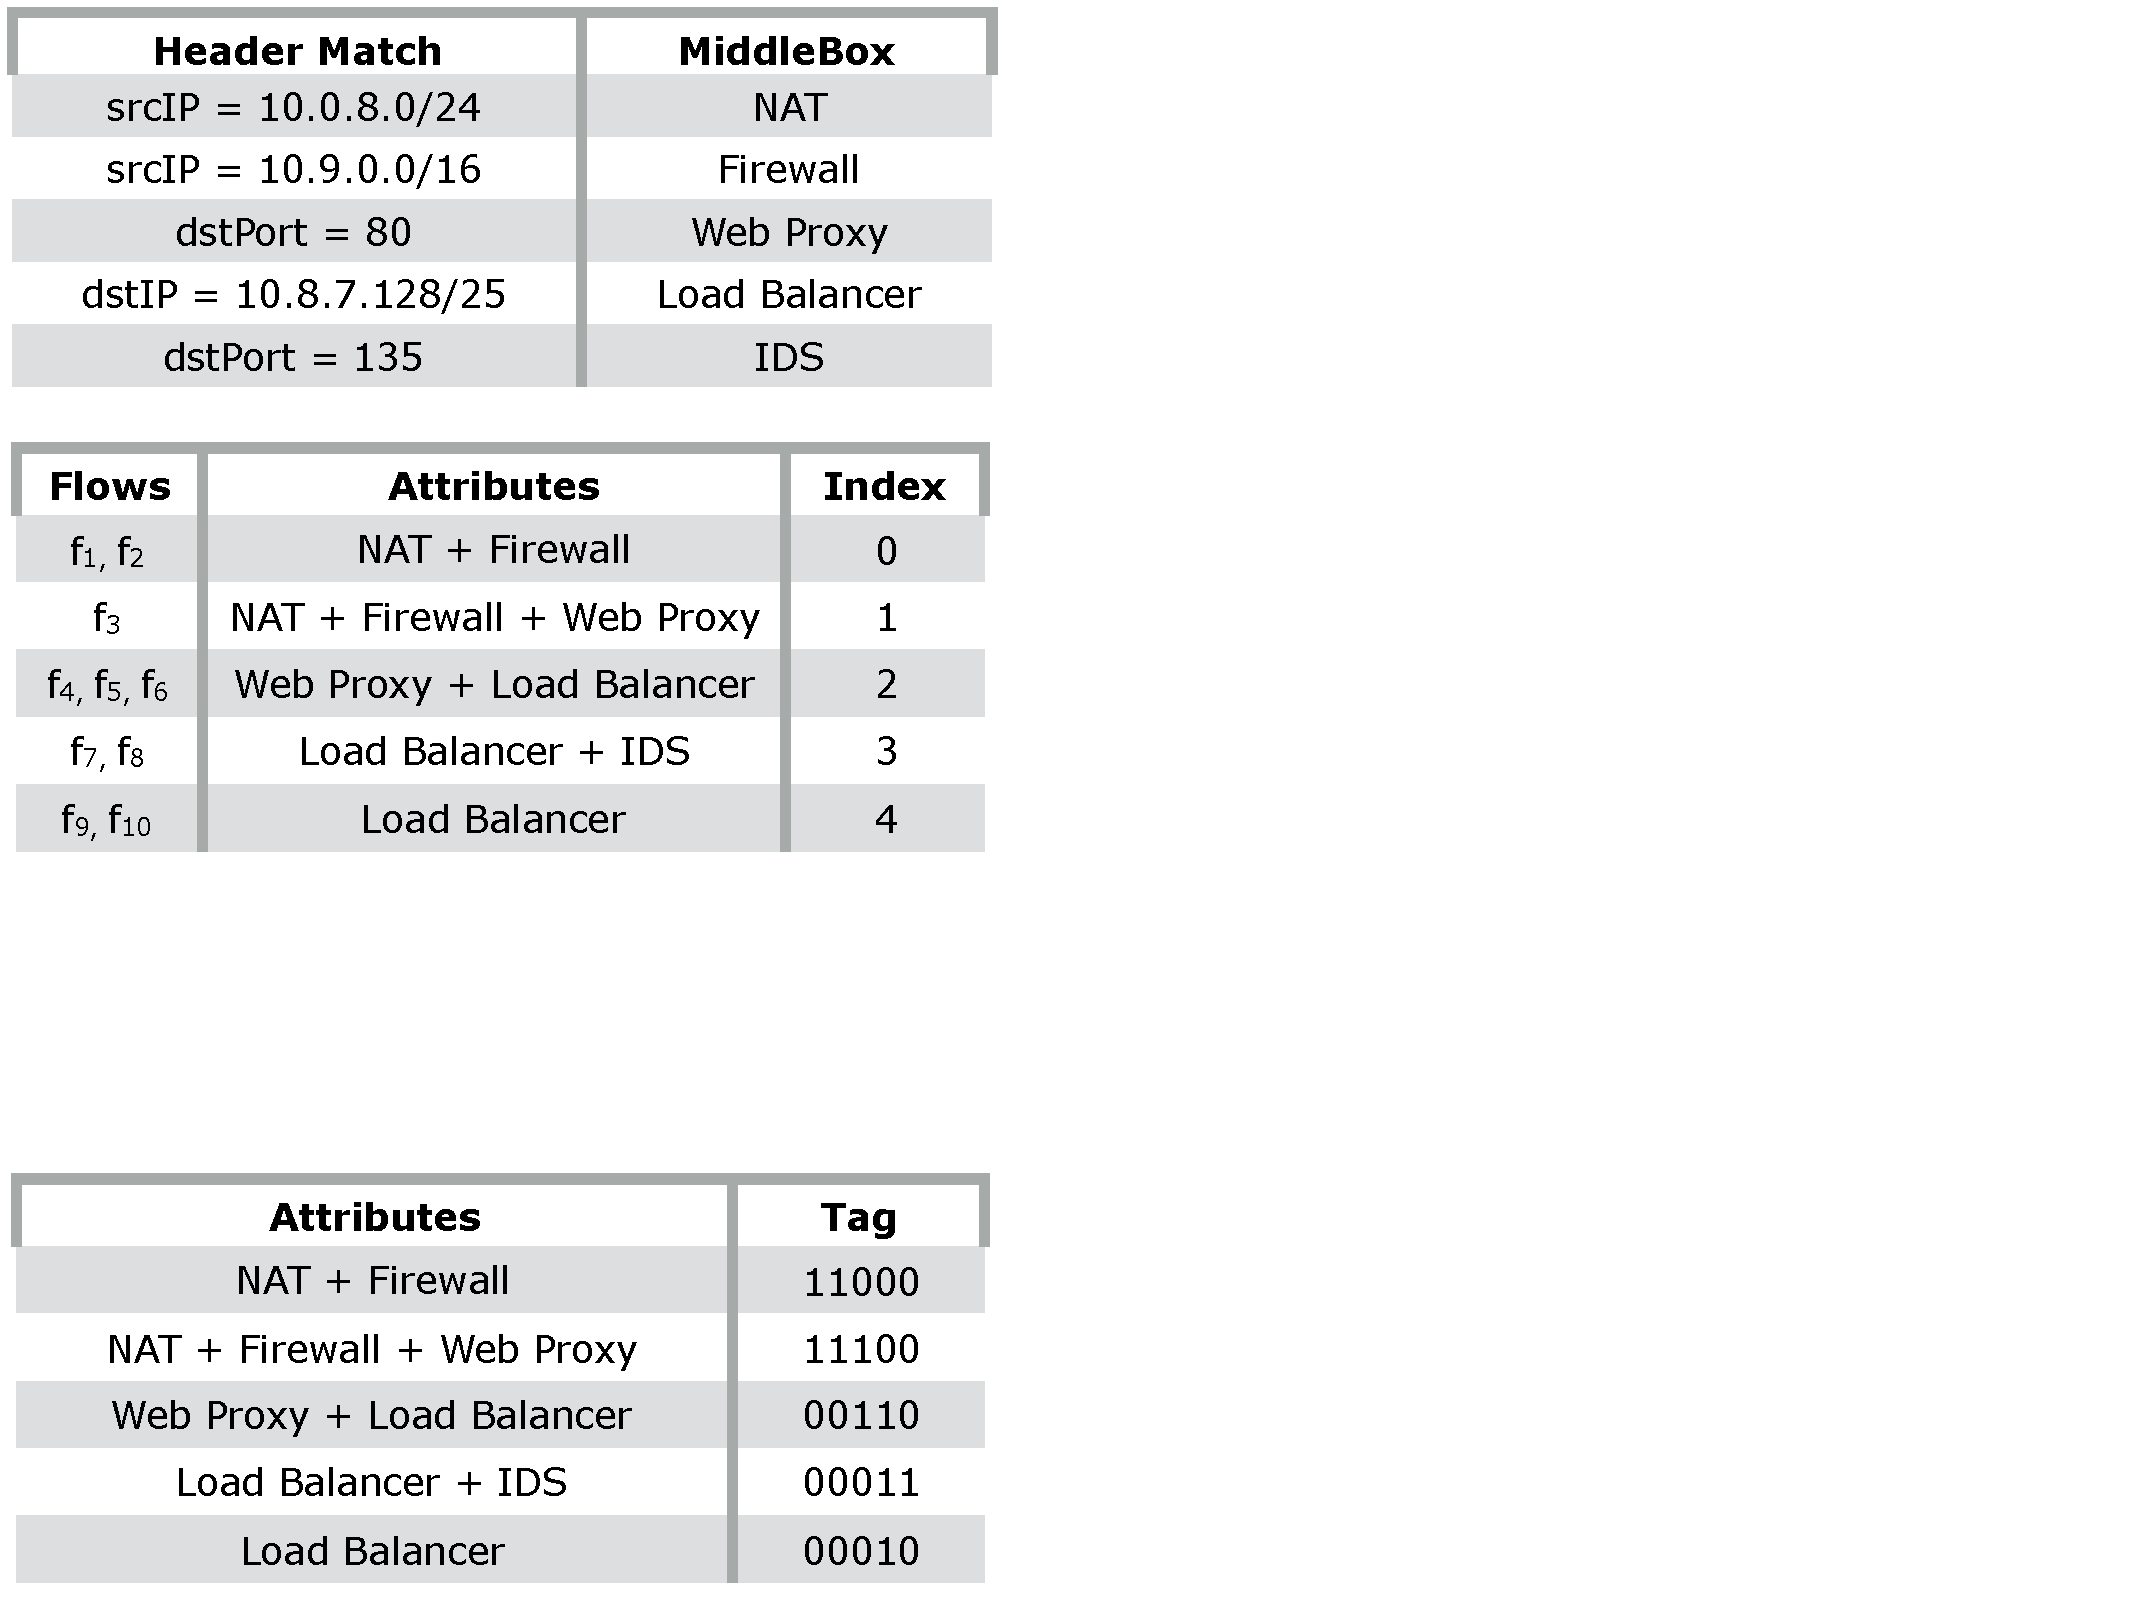
\includegraphics[trim={0 0 19cm 19.5cm}, clip, width=\linewidth]{figures/mbox_path_example3}
\end{subfigure} 
\end{minipage} 
\caption{A simple attribute-carrying tag format for the service chaining example. Each middlebox is mapped to a bit in the tag, and that bit is 1 if the middlebox must be traversed.}
\label{fig:att_tags}
\end{figure}

Attribute reading need not be so complex, though. If we do not require optimal tag width, we can construct tags such that the attributes are more quickly read. Figure \ref{fig:att_tags} shows such a construction for service chains, with tags as bitfields. Each attribute can be read using a single wildcard match, but the tag width is equal to the number of middleboxes. It is interesting to note that when each bitfield tag is viewed as an integer, it can still be thought of as an index into a implicit table of all possible attribute sets. 
%%%%%%%%%%%%%%%%%%%%%%%%%%%


\subsection{Motivating Applications}
There are many applications where a forwarding equivalence class is characterized by a distinct set of attributes, and where the switches could benefit from being able to read these sets using a small amount of memory. To motivate our solution, we will present four such applications. 

\subsubsection{Software-Defined Internet Exchange Points}
Consider the example of an Internet Exchange Point (IXP) with support for SDN policies. At such an IXP, connected networks may wish to apply SDN policies to their traffic as it enters the exchange point. If these policies were not present, all traffic from some network $P$  to some destination IP prefix $d$ would be directed to the BGP default next-hop for $d$ as decided by $P$. In the presence of SDN policies, however, traffic may be redirected to take a next-hop which differs from the BGP default next-hop. For correctness, this redirection must be to a next-hop which has announced a route to $d$ , and $P$'s policies must take this into account. If it were possible to attach to each packet leaving $P$ the set of next-hops which have advertised $d$ to $P$, policies could check for the presence of a next-hop in the set before rerouting the packet to that next-hop. 

\subsubsection{Service Chaining}
For another example, network operators often desire that network traffic be directed through a series of middleboxes, such as load balancers or firewalls. Such middleboxes can provide security and performance guarantees for the network's users. However, each flow may need to be directed through a different chain of middleboxes. In this case, the set of attributes which define an equivalence class would be a chain of middleboxes. Switches could check for the presence of a middlebox attribute in the FEC tag and, if present, forward that flow towards the nearest matching middlebox. This could be accomplished with an MPLS label stack, but middleboxes do not necessarily understand or preserve MPLS labels. 

\subsubsection{Host Attributes for Network Policies}


\subsubsection{Multicast and Anycast}
For another example, consider the case of anycast. In traditional anycast, many receivers are identified by the same address, and each anycast packet simply chooses the nearest receiver according to some distance metric. There is no flexibility for selecting arbitrary subsets of hosts without applying the same identifier to the subset of receivers. We envision the potential for a more flexible local area network anycast, where each packet can be mapped to an arbitrary subset of hosts, regardless of their addresses. If it were possible to tag each packet during classification with a list of host identifiers, switches could read this list and pick the nearest for forwarding.